% !TEX root = ../thesis.tex
\chapter{Preliminaries}
\label{sec:definitions}

In this chapter we will define concepts that are used in \Cref{sec:behaviours} to reason about the implemented runtime.

While the \gls{tessla} specification itself defines a set of semantics, for this thesis we will slightly alter some of it and add some new definitions based on them.
This is necessary to reason about the specifics how the runtime is built (Note that \gls{tessla} doesn't define an operational semantic, therefore we will define our own) and how it behaves.

\section{Time}
\label{sec:definitions:time}

\gls{tessla} has a model of continuous time, where timestamps \(\pi \in \mathbb{T} \) are used to represent a certain point in time and \(\mathbb{T}\) has to be isomorphic to \(\mathbb{R}\).

\section{Transducers}
\label{sec:definitions:transducers}

Fundamentally \gls{tessla} is a special kind of a transducer.
Therefore in this section we will define a model of transducers which can be used to reason about the evaluation of a \gls{tessla} specification.

A transducer is a system, which consumes an input and produces an output.
Let \(\Phi, \Gamma\) be two alphabets and \(\epsilon\) the empty word.

\begin{definition}[name = Transducer]\label{def:transducer}
  A transducer \(t\) is a relation \(t \subseteq \Phi^* \times \Gamma^*\), \(\Phi\) is called the input alphabet, \(\Gamma\) the output alphabet.
\end{definition}

\gls{tessla} specifications are deterministic for any input, meaning they should produce the same output for the same input.

\begin{definition}[name = Deterministic Transducer]\label{def:deterministic_transducer}
  A deterministic transducer relates each input to at most one output.
\end{definition}

\begin{exmp}[name = Deterministic and Nondeterministic Transducers]
  \(t_d = \{(a,1),(b,2),(ab,12),(ba,21)\}\) is a deterministic transducer, \(t_{nd} = \{(a,1),(a,2)\}\) is nondeterministic, because it relates input \(a\) to both outputs \(1\) and \(2\).
\end{exmp}

Transducers can furthermore be categorized as synchronous, asynchronous, causal and clairvoyant transducers:
synchronosity is a property over the behaviour of a transducer when it's consuming input per element.
If it is synchronous, it will produce an output element for each input element.

\begin{definition}[name = Synchronous Transducer]\label{def:synchronous_transducer}
Let \(\vec{\imath} \in \Phi^*, i \in \Phi, \vec{o} \in \Gamma^*, o \in \Gamma\).
  A transducer \(t\) is called synchronous, when it satisfies, that:
  if \( (\vec{\imath}\circ i,\vec{o}\circ o) \in t\)
  then \( (\vec{\imath}, \vec{o}) \in t \)
\end{definition}

An asynchronous transducer can produce zero, one or many outputs for each input it consumes.

\begin{definition}[name = Asynchronous Transducer]\label{def:asynchronous_transducer}
  Let \(\vec{\imath}\in \Phi^*, i \in \Phi,\vec{o} \in \Gamma^*\).
  A transducer \(t\) is called asynchronous when it satisfies the formula:
  if \((\vec{\imath}\circ i, \vec{o}) \in t \)
  then \(\exists \vec{o'},\vec{o''} \in \Gamma^*\text{ so that } \vec{o} = \vec{o'}\circ\vec{o''} \text{ and } (\vec{\imath},\vec{o'}) \in t \)
\end{definition}

\begin{exmp}[name = Synchronous and Asynchronous Transducers]
  \(t_s = \{(a,1),(b,2),(ab,12),(ba,21)\}\) is a synchronous transducer, \(t_{as} = \{(a,\epsilon),(ab,12)\}\) is asynchronous.
\end{exmp}

A causal transducer is one, where the output depends only on consumed inputs and not on future inputs:

\begin{definition}[name = Causal and Clairvoyant Transducers]\label{def:causal_transducer}
  A transducer \(t\) is called causal, when it satiesfies, that:
  if \((\vec{\imath},\vec{o}) \in t \)
  then \( \forall \vec{\imath'} \in \Phi^* \text{ with } (\vec{\imath} \circ \vec{\imath'}, \vec{o'}) \in t \)
  it holds, that \( \vec{o} \sqsubseteq \vec{o'} \)

  A transducer that isn't casual is called \emph{clairvoyant}.
\end{definition}


\begin{exmp}[name = Causal and Clairvoyant Transducers]
  \(t_{cl} = \{(a,1),(b,2),(ab,12),(ba,21)\}\) is a causal transducer, because each output only depends on the inputs seen upto that point, \(t_{cl} = \{(a,1),(ab,22),(aa,11)\}\) is clairvoyant, because the output when the letter \(a\) is seen depends on the next input.
\end{exmp}

When talking about transducers, it is interesting to know if two transducers are \emph{equivalent}.
There are multiple possible definitions for equivalence of transducers, we will look at two, which are interesting for this thesis.
In the following \(\sigma_i\) is used to get the element at position \(i\) and \(\sigma_{[i,j]}\) to get the infix of \(\sigma\) which starts at position \(i\) and ends at position \(j\) (With \(0\) as the index of the first element).

\begin{definition}[name = Asynchronous equivalence of Transducers]\label{def:async_equivalence_transducer}
  Let \(t_1, t_2\) be two asynchronous transducers from \(\Phi^*\) to \(\Gamma^*\).
  They are called \emph{asynchronous equivalent}, written \(t_1 \equiv_a t_2\), if they satisfy: \\
  \(\forall \sigma \in \Phi^*\):
  \begin{itemize}
    \item \(\forall (\sigma_{[0,k]}, \vec{o}) \in t_1\): \(\exists k' \geq k \text{ with } (\sigma_{[0,k']}, \vec{o'}) \in t_2\) and \(\vec{o} \sqsubseteq \vec{o'}\)
    \item and \(\forall (\sigma_{[0,k]}, \vec{o}) \in t_2\): \(\exists k' \geq k \text{ with } (\sigma_{[0,k']}, \vec{o'}) \in t_1\) and \(\vec{o} \sqsubseteq \vec{o'}\)
  \end{itemize}
\end{definition}

\begin{lemma}[name=Asynchronous equivalence is an equivalence Relation]\label{lemma:async_equivalence_is_equivalence_relationship}
  Asynchronous equivalence is symmetric, reflexive and transitive.
\end{lemma}

\begin{proof}
    Symmetry is trivial, since the second part of the definition is requiring it.\\
    Reflexivity is also trivial, for \((\sigma_{[0,k]}, \vec{o})\) select \(k' = k\).\\
    For transitivity:
    \begin{itemize}[label = {}]
      \item Let \(t_1 \equiv_a t_2\), \(t_2 \equiv_a t_3\).
      \item First case:
        \begin{align*}
          &\text{Since } t_1 \equiv_a t_2:\ \forall (\sigma_{[0,k_1]}, \vec{o_1}) \in t_1: \\
          &\hspace{2em} \exists k_2\ \text{such, that } (\sigma_{[0,k_2]}, \vec{o_2}) \in t_2\ \text{with } \vec{o_1} \sqsubseteq \vec{o_2} \\
          &\hspace{2em} \text{and since } t_2 \equiv_a t_3 \\
          &\hspace{4em} \exists k_3\ \text{such, that } (\sigma_{[0,k_3]}, \vec{o_3}) \in t_3\ \text{with } \vec{o_2} \sqsubseteq \vec{o_3}\\
          &\hspace{4em} \text{With } \vec{o_1} \sqsubseteq \vec{o_2} \sqsubseteq \vec{o_3}\ \text{it follows, that } t_1 \equiv_a t_3
        \end{align*}
      \item The second case works the same, just change \(t_1\) and \(t_3\).
    \end{itemize}
\end{proof}

\begin{exmp}[name = Asynchronous equivalence of Transducers]
  Let \(\Phi = \{a\}, \Gamma = \{1\}\) and \\
  \begin{align*}
    &t_1 = \{&&(a,\epsilon),  &&(aa,\epsilon),  &&(aaa,111)   &\} \\
    &t_2 = \{&&(a,1),         &&(aa,1),         &&(aaa,111)   &\} \\
    &t_3 = \{&&(a,\epsilon),  &&(aa,1),         &&(aaa,11)    &\}\\
  \end{align*}
  All three transducers are asynchronous and causal.
  Let's see which ones are asynchronous equivalent:

  \(t_1 \stackrel{?}{\equiv}_a t_2\)
  \begin{align*}
    &(a,\epsilon)  &&\in t_1, k = 1 &\rightarrow k' = 1, &(a,1)     \in t_2, &\epsilon  &\sqsubseteq 1 \\
    &(aa,\epsilon) &&\in t_1, k = 2 &\rightarrow k' = 2, &(aa,1)    \in t_2, &\epsilon  &\sqsubseteq 1 \\
    &(aaa,111)     &&\in t_1, k = 3 &\rightarrow k' = 3, &(aaa,111) \in t_2, &111       &\sqsubseteq 111 \\
    &(a,1)         &&\in t_2, k = 1 &\rightarrow k' = 3, &(aaa,111) \in t_1, &1         &\sqsubseteq 111 \\
    &(aa,1)        &&\in t_2, k = 2 &\rightarrow k' = 3, &(aaa,111) \in t_1, &1         &\sqsubseteq 111 \\
    &(aaa,111)     &&\in t_2, k = 3 &\rightarrow k' = 3, &(aaa,111) \in t_1, &111       &\sqsubseteq 111 \\
  \end{align*}
  \(\Rightarrow t_1 \equiv_a t_2\)

  \(t_1 \stackrel{?}{\equiv}_a t_3\)
  \begin{align*}
    &(aaa,111)     \in t_1, k = 3 \rightarrow \not\exists k'
  \end{align*}
  \(\Rightarrow t_1 \not\equiv_a t_3\)

  Because of \Cref{lemma:async_equivalence_is_equivalence_relationship} \(\Rightarrow t_2 \not\equiv_a t_3\).

\end{exmp}

\section{Timed Transducers}
\label{sec:definitions:timed_transducer}

For the second kind of equivalence we need to introduce \emph{timed sequences}, originally introduced as timed words in~\cite{Alur1994}, and \emph{timed transducers}.
Note that timed sequences don't have to be monotonically increasing like in the original definition.
Quite on the contrary the unorderdness of outputs is an important key principle to much of the later work as you will see.

Let \(\mathbb{T}\) be a timing model that is isomorphic to \(\mathbb{R}\).
For the examples we will use \(\mathbb{R}\) for \(\mathbb{T}\).

\begin{definition}[name = Timed Sequence]\label{def:timed_sequence}
  A sequence is called timed, if every element of it is associated with a timestamp: \(\sigma \in {(\Gamma\times\mathbb{T})}^*\).
  For bravety a timed sequence can be written with the timestamps as the index of the elements: \(\sigma = e_0e_{0.5}e_1 \).\\
  The function
  \[\mathit{timed: } {(\Gamma \times \mathbb{T})}^* \rightarrow {(\Gamma \times \mathbb{T})}^* \]
  reorders a timed sequence \(\sigma\) by its timestamps, such that:
  \[ \forall i,j \in \mathbb{N}:\text{ if } i < j \text{ then } \pi_i < \pi_j \text{ with } (o_i, \pi_i) = \sigma_i \text{ and } (o_j, \pi_j) = \sigma_j \]
  The function
  \[\mathit{upto: } \mathbb{T} \times {(\Gamma\times\mathbb{T})}^* \rightarrow {(\Gamma\times\mathbb{T})}^*\]
  removes all elements from a timed sequence, that have a timestamp bigger than the first argument.\\
  The function
  \[\mathit{maxTime: } {(\Gamma\times\mathbb{T})}^* \rightarrow \mathbb{T} \]
  returns the biggest Timestamp in a timed sequence.
\end{definition}

\begin{exmp}[name=Functions on Timed Sequences]
Let \(\sigma = a_1a_{0.5}a_{1.5}a_0\).\\
  Then is
    \begin{align*}
      &\mathit{timed} (\sigma) = a_0a_{0.5}a_1a_{1.5}\ \\
      &\mathit{upto} (1.3,\sigma) = a_1a_{0.5}a_0 \\
      &\mathit{maxTime} (\sigma) = 1.5
    \end{align*}
\end{exmp}

\begin{definition}[name = Monotonicity of Timed Sequences]\label{def:monotonicity_timed_sequences}
  A timed sequence \(\sigma\) with alphabet \(\Phi\) is called monotonic,
  if \( \mathit{timed}(\sigma) = \sigma\)
\end{definition}

\begin{definition}[name = Timed Transducer]\label{def:timed_transducer}
  A timed transducer \(t\) with input alphabet \(\Phi\) and output alphabet \(\Gamma\) works on monotonic, timed sequences as inputs and has timed sequences as outputs:
  \[t \subset {\left(\Phi \times \mathbb{T}\right)}^* \times {\left(\Gamma \times \mathbb{T}\right)}^*\]
\end{definition}

\begin{exmp}[name=Timed Transducers]
  \begin{align*}
    &\text{Let } \Phi = \{a\}, \Gamma = \{b\}.\\
    &t_{tsc} = \{(a_0, b_0),(a_0a_1, b_0b_1)\}\ \text{is a timed, causal and synchronous transducer.}\\
    &t_{tac} = \{(a_0, \epsilon),(a_0a_1, b_0b_1)\}\ \text{is a timed, causal and asynchronous transducer.}
  \end{align*}
\end{exmp}

For later theoretic work we have to restrict timed transducers.

\begin{definition}[name = Boundedness of Timed Transducers]\label{def:boundedness_timed_transducer}
  A timed transducer \(t\) with input alphabet \(\Phi\) and output alphabet \(\Gamma\) is called bounded, if it satisfies:
  \begin{align*}
    &\forall \sigma \in {(\Phi \times \mathbb{T})}^*:\\
    &\hspace{2em}\text{if } (\sigma_{[0,k]}, \vec{o}) \in t\\
    &\hspace{2em}\text{then }\exists k' > k\ \text{with}\\
    &\hspace{4em}(\sigma_{[0,k']}, \vec{o} \circ \vec{o'}) \in t\\
    &\hspace{4em}\text{and} \forall k'' > k'\ \text{with } (\sigma_{[0,k'']}, \vec{o}\circ\vec{o'}\circ\vec{o''}) \in t\ \text{it holds, that}\\
    &\hspace{6em}\mathit{upto}(\mathit{maxTime}(\vec{o}), \mathit{timed}(\vec{o}\circ\vec{o'})) = \mathit{upto}(\mathit{maxTime}(\vec{o}), \mathit{timed}(\vec{o}\circ\vec{o'}\circ\vec{o''}))
  \end{align*}
\end{definition}
Based on the definitions we can define an equivalence relationship on bounded timed transducers.

\begin{definition}[name = Observational Equivalence]\label{def:observational_equivalence}
  Let \(t_1, t_2\) be two bounded timed transducers with input alphabet \(\Phi\) and output alphabet \(\Gamma\).
  They are called \emph{observational equivalent}, written \(t_1 \equiv_o t_2\), if they satisfy:
  \begin{align*}
    &\forall \sigma \in {(\Phi\times\mathbb{T})}^*:\\
    &\hspace{2em}\forall (\sigma_{[0,k]}, \vec{o}) \in t_1: \exists k', k'' \geq k\ \text{such that}\\
    &\hspace{4em}(\sigma_{[0,k']}, \vec{o} \circ \vec{o'}) \in t_1\\
    &\hspace{4em}\text{and } (\sigma_{[0,k'']}, \vec{o_2}) \in t_2\\
    &\hspace{4em}\text{and } \mathit{timed}(\mathit{upto}(\mathit{maxTime}(\vec{o}),\vec{o} \circ \vec{o'} )) = \mathit{timed}(\mathit{upto}(\mathit{maxTime}(\vec{o}),\vec{o_2}))
  \end{align*}
  and the same for switched \(t_1, t_2\).
\end{definition}

What does observational equivalence between two transducers intuitively mean?
It means that two transducers eventually produce the same output values for the same timed inputs, maybe in a different order, but with the same timestamps, which is very important.
Since the values are associated with timestamps the outputs can be reordered by them and therefore be exactly equal.

\begin{lemma}[name=Observational Equivalence is an Equivalence Relationship for Bounded Transducers]\label{lemma:observational_equivalence_equivalence_relationship}
  \(\equiv_o\) is symmetric, reflexive and transitive for bounded timed transducers.
\end{lemma}
\begin{proof}
  Let \(t_1, t_2, t_3\) be bounded timed transducers.
  Symmetry follows directly from the definition.\\
  Reflexivity: For \((\sigma_{[0,k]}, \vec{o})\) select \(k' = k''\) as the k, for which the transducer is bounded for that input.\\
  Transitivity:
  \begin{itemize}
    \item Let \(t_1 \equiv_o t_2\), \(t_2 \equiv_o t_3\).
    \item First case:
      \begin{alignat*}{2}
        &\text{Since } t_1 \equiv_o t_2:\ \forall (\sigma_{[0,k_1]}, \vec{o_1}) \in t_1: \\
        &\hspace{2em} \exists k_1', k_2 > k_1\ \text{with } (\sigma_{[0,k_1']}, \vec{o_1}\circ\vec{o_1'}) \in t_1\ \text{and } (\sigma_{[0,k_2]}, \vec{o_2}) \in t_2 \\
        &\hspace{4em} \text{with } \mathit{timed}(\mathit{upto}(\mathit{maxTime}(\vec{o_1}),\vec{o_1} \circ \vec{o_1'} )) \\
        &\hspace{8em} = \mathit{timed}(\mathit{upto}(\mathit{maxTime}(\vec{o_1}),\vec{o_2})) && (\star)\\
        &\hspace{2em} \text{and since } t_2 \equiv_o t_3: \exists k_2', k_3 > k_2\ \text{with } (\sigma_{[0,k_2']}, \vec{o_2}\circ\vec{o_2'}) \in t_2 \\
        &\hspace{4em} \text{and } (\sigma_{[0,k_3]}, \vec{o_3}) \in t_3 \\
        &\hspace{6em} \text{with } \mathit{timed}(\mathit{upto}(\mathit{maxTime}(\vec{o_2}),\vec{o_2} \circ \vec{o_2'} )) \\
        &\hspace{10em} = \mathit{timed}(\mathit{upto}(\mathit{maxTime}(\vec{o_2}),\vec{o_3})) && (\star\star)\\
        &\hspace{2em} \mathit{maxTime}(\vec{o_1})\ \text{has to be smaller than }\mathit{maxTime}(\vec{o_2}), \\
        &\hspace{2em} \text{else } (\star)\ \text{couldn't hold, therefore, combined with boundedness and }(\star\star): \\
        &\hspace{4em} \mathit{timed}(\mathit{upto}(\mathit{maxTime}(\vec{o_1}),\vec{o_2} )) \\
        &\hspace{8em} = \mathit{timed}(\mathit{upto}(\mathit{maxTime}(\vec{o_1}),\vec{o_3})) \\
        &\text{which concludes }\mathit{timed}(\mathit{upto}(\mathit{maxTime}(\vec{o_1}),\vec{o_1} \circ \vec{o_1'} ))\\
        &\hspace{4em} = \mathit{timed}(\mathit{upto}(\mathit{maxTime}(\vec{o_1}),\vec{o_3}))
      \end{alignat*}
    \item The second case works the same, just switch \(t_1\) and \(t_3\).
  \end{itemize}
\end{proof}


\begin{exmp}[name=Observational Equivalence]\label{exmp:observational_equivalence}
  Let
  \begin{align*}
    &t_1 = \{&&(a_0, \epsilon),   &&(a_0a_1, b_1),      &&(a_0a_1a_2, b_1b_2b_0)  &\} \\
    &t_2 = \{&&(a_0, \epsilon),   &&(a_0a_1, \epsilon), &&(a_0a_1a_2, b_2b_1b_0)  &\} \\
    &t_3 = \{&&(a_0, b_0),        &&(a_0a_1, b_0),      &&(a_0a_1a_2, b_2b_1)     &\}
  \end{align*}
  All three are causal, asynchronous timed transducers.

  Let's see which ones are observational equivalent:

  \(t_1 \stackrel{?}{\equiv}_o t_2\)
  \begin{itemize}[label={}]
    \item \((a_0, \epsilon)             \in t_1, k = 1, \mathit{maxTime}(\epsilon) = 0\)
      \begin{itemize}[label={}]
        \item \(\rightarrow k' = 1, (a_0, \epsilon)     \in t_1\)
        \item \(\rightarrow k'' = 1, (a_0, \epsilon)     \in t_2\)
      \end{itemize}
    \item \((a_0a_1, b_1)               \in t_1, k = 2, \mathit{maxTime}(b_1) = 1\)
      \begin{itemize}[label={}]
        \item \(\rightarrow k' = 3, (a_0a_1a_2, b_1b_2b_0)    \in t_1\)
        \item \(\rightarrow k'' = 3, (a_0a_1a_2, b_2b_1b_0)    \in t_2\)
        \item \(\mathit{timed}(\mathit{upto}(1, b_1b_2b_0)) = b_0b_1 = \mathit{timed}(\mathit{upto}(1, b_2b_1b_0))\)
      \end{itemize}
    \item \((a_0a_1a_2, b_1b_2b_0)               \in t_1, k = 3, \mathit{maxTime}(b_1b_2b_0) = 2\)
      \begin{itemize}[label={}]
        \item \(\rightarrow k' = 3, (a_0a_1a_2, b_1b_2b_0)    \in t_1\)
        \item \(\rightarrow k'' = 3, (a_0a_1a_2, b_2b_1b_0)    \in t_2\)
        \item \(\mathit{timed}(\mathit{upto}(2, b_1b_2b_0)) = b_0b_1b_2 = \mathit{timed}(\mathit{upto}(2, b_2b_1b_0))\)
      \end{itemize}
    \item \((a_0, \epsilon)               \in t_2, k = 1, \mathit{maxTime}(\epsilon) = 0\)
      \begin{itemize}[label={}]
        \item \(\rightarrow k' = 1, (a_0, \epsilon)     \in t_2\)
        \item \(\rightarrow k'' = 1, (a_0, \epsilon)     \in t_1\)
      \end{itemize}
    \item \((a_0a_1, \epsilon)            \in t_2, k = 2, \mathit{maxTime}(epsilon) = 0\)
      \begin{itemize}[label={}]
        \item \(\rightarrow k' = 2, (a_0a_1, \epsilon)    \in t_2\)
        \item \(\rightarrow k'' = 2, (a_0a_1, b_1)    \in t_1\)
        \item \(\mathit{timed}(\mathit{upto}(0, \epsilon)) = \epsilon = \mathit{timed}(\mathit{upto}(0, b_1))\)
      \end{itemize}
    \item \((a_0a_1a_2, b_2b_1b_0)        \in t_2, k = 3, \mathit{maxTime}(b_2b_1b_0) = 2\)
      \begin{itemize}[label={}]
        \item \(\rightarrow k' = 3, (a_0a_1a_2, b_2b_1b_0)    \in t_2\)
        \item \(\rightarrow k'' = 3, (a_0a_1a_2, b_1b_2b_0)    \in t_1\)
        \item \(\mathit{timed}(\mathit{upto}(2, b_2b_1b_0)) = b_0b_1b_2 = \mathit{timed}(\mathit{upto}(2, b_1b_2b_0))\)
      \end{itemize}
  \end{itemize}
  \(\Rightarrow t_1 \equiv_a t_2\)

  \(t_1 \stackrel{?}{\equiv}_a t_3\)
  \begin{itemize}[label={}]
    \item \((a_0a_1a_2,b_1b_2b_0)      \in t_1, k=3, \mathit{maxTime}(b_1b_2b_0) = 2\)
      \begin{itemize}[label={}]
        \item \(\rightarrow k' = 3, (a_0a_1a_2, b_1b_2b_0)    \in t_1\)
        \item \(\rightarrow \not\exists (\vec{\imath}, \vec{o}) \in t_3\ \text{with } \exists n \in \mathbb{N}: \vec{o}_n = b_0\)
        \item \(\rightarrow \not\exists (\vec{\imath}, \vec{o}) \in t_3\ \text{with } \mathit{timed}(\mathit{upto}(2, b_1b_2b_0)) = b_0b_1b_2 = \mathit{timed}(\mathit{upto}(2,\vec{o}))\)
      \end{itemize}
  \end{itemize}
  \(\Rightarrow t_1 \not\equiv_a t_3\)\\
  If \(t_3\) weren't bounded (and therefore not finite) there would be no way to know, if it was equivalent to \(t_1\), because it could always produce a missing event at a later time.

  Because of \Cref{lemma:observational_equivalence_equivalence_relationship} \(\Rightarrow t_2 \not\equiv_a t_3\).

\end{exmp}

% \section{Labeled Timed Transducers}
% Maybe necessary, maybe not

\section{Events}
\label{sec:definitions:events}

Events are the atomic unit of information that all computations are based on.
There are three types of events: external, output and internal events.

The set of all events is denoted as \(E\).
Each event carries a value, which can be \emph{nothing} or a value of a type (types are formally defined in the \gls{tessla} specification, but aren't important for this thesis), a timestamp and the stream it's perceived on (for example a function call of a specific function or the name of an output stream).

The value of an event can be queried with the function \(\upsilon\), its timestamp with \(\mathit{time}\) and its stream with \(\mathit{stream}\).

\(E_e \subset E\) is the set of all external events, their stream corresponds to a specific trace.
\(E_o \subset E\) is the set of all output events, their stream is specified by an output name of the \gls{tessla} specification.
\(E_n \subset E\) is the set of all internal events.
Internal events are mostly an implementation detail, which denote steps of computation inside the runtime.
The stream of internal events is implicitly given by the node that produces the stream of the event.
Note that \(E_e, E_o, E_n\) are pairwise disjoint and \(E_e \cup E_o \cup E_n = E\).

\section{Streams}
\label{sec:definitions:streams}

Streams are a collection of events with specific characteristics.
While events are the atomic unit of information, streams represent the sequence of related events over time.

There are two kind of streams: signals, which carry values at all times, and event\-streams, which only hold values at specific times.
Eventstreams can be described by a sequence of events.
Signals can be described by a sequence of changes, where a change denotes that the value of a signal changed at a specific timestamp.
The only difference between a signal and an eventstreams is that signals always have a value while an eventstream may return \(\bot\) when queried for its value at a specific time, which denotes that no event happened at that time.
Based on the similarity of signals and eventstreams in the following we will mainly reason about eventstreams, but most things can also be applied to signals.

Formally a stream \(\sigma\) can be represented as the product of a sequence of events \(\langle e_1, \dots e_n\rangle\) where \(\mathit{time}(e_i) < \mathit{time}(e_{i+1}),\ \forall i < n \in \mathbb{N}\).
The set of all streams \(\Sigma\) is defined as all possible finite sequences of events \(\Sigma = \{\sigma | \sigma \in E^* \}\).
An external stream \(\sigma_e\) is a stream consisting only of external events, the set of all external streams is \(\Sigma_e = \{\sigma_e | \sigma_e \in E_e^*\} \times \mathbb{T}\).
Output and internal streams are defined analogous.

To get the event of a stream \(\sigma\) at a timestamp \(\pi\) it can be queried like a function: \(\sigma(\pi) = e\) with \(\mathit{time}(e) = \pi \).
When working with signals, the function will return the latest event that happened at or before t while an eventstream may return \(\bot\).
The progress of a stream, which is the timestamp of the last event that happened on them, can be obtained with \(\mathit{progress}(\sigma) = \pi \in \mathbb{T}\).
Internal and output streams can be queried for the node that produced them with \(\mathit{node}(\sigma) = n \in N\).

\section{Functions}
\label{sec:definitions:functions}

A \gls{tessla} specification consists of functions over streams.
Functions generate new streams by applying an operation on existing streams.
\gls{tessla} itself defines a syntax to write a specification, a set of types and a standard library of functions, but an implementation is free to choose the functions it supports.

An example function is \(\mathit{add}(S_D,S_D) \rightarrow S_D\): It takes two signals, which have to hold values of some numerical type, and produces a signal which holds values of the same type.
The produced stream can either be assigned to a named identifier (think: a variable) or consumed by another function (function composition).

Functions can be divided into three categories: pure, unpure and timing.
Pure functions, also called stateless, are evaluated only on the values their inputs have at the timestamp they are evaluated, therefore they don't have to remember a state and will only return events.
Unpure, or stateful, functions are evaluated over the values if its inputs at that timestamp and a state and will return not only new events but also an updated state.
As an example a function \emph{eventCount} has to \emph{remember} how many events already happened on it's input stream and increment that counter on every new event.
Timing functions are evaluated not only on the value of events but also on their timestamp and can also manipulate it:
While non timing functions will consume events at a specific timestamp and emit events with that timestamp, timing functions can emit events with a changed timestamp.
In this thesis we will only look at past time functions, meaning functions can only delay timestamps, therefore can't depend on future values.

Timing functions complicate the reasoning about schedules and causality and therefore aren't included in \Cref{sec:behaviours:without_timing}.
In \Cref{sec:behaviours:timing_functions} the conclusions of earlier sections will be extended to include timing functions.

\section{Nodes}
\label{sec:definitions:nodes}

Nodes are the atomic unit of computation for the evaluation of a \gls{tessla} specification.
A node implements a single function: there is an \emph{AddNode} which takes two input signals and produces a new signal.
Therefore a node is the concrete implementation of a function in a runtime for \gls{tessla} specifications.
The set of all nodes is called \(N\).
The function of a node \(n \in N\) is written as \(f_n\).

Each node has a set of inputs, which are either external or internal streams, and one output, which is either an internal or an output stream.
Nodes which have at least one external stream as an input are called \emph{sources}.
Nodes have a state, described in \Cref{sec:definitions:state}, which contains \gls{fifo} queues, provided by the Erlang platform, which buffer events from its inputs for later computation.

Every new event added to a queue has to have a bigger timestamp than the previous event added to the queue.
This means a queue has a kind of progress timestamp, which denotes the timestamp of the latest event added to it and which is strictly increasing over time.
Queues support the standard operators for lists like \(\mathit{hd}, \mathit{tl}, ++\) to respectively get the head, the tail or to append to the end.


\section{\glsentryname{tessla} Evaluation Engine}
\label{sec:definitions:eval_engine}

Because functions in \gls{tessla} specifications depend on other functions, and these dependencies have to be cycle free, the specification can be represented as a \gls{dag}, where the functions are vertices and the relationship between functions are edges.
This is exactly how the \gls{tessla} compiler outputs a specification.
One can now use the \gls{dag} of a \gls{tessla} specification to synthesize a system to evaluate it over inputs:
The vertices of the \gls{dag} become nodes representing the functions and the edges are the input and output streams between the nodes.
We will call this synthesized system an \emph{evaluation engine}.

When fed with inputs (or \emph{traces}) the engine will produce outputs.
The relationship between inputs and outputs that is produced can be seen as a timed transducer.
The input to an evaluation engine has to have strictly increasing timestamps.
This is needed to have a known progress which can be distributed through the system.
If inputs weren't ordered by their timestamp for example the absense of input events on a specific stream couldn't be detected because events could be present at a later position of the input trace.
Especially for offline monitoring this obviously is no problem because the traces can simply be reordered into a strictly increasing sequence, except when multiple input events are at the same timestamp.
This can be solved in two ways: either increase the timing precision when generating the traces or manipulate the timestamps in the traces by adding a minimal offset to them if they are equal to another timestamp.

To evaluate a specification over traces, the evaluation engine has process the events that were traced.
To do so the nodes have to run their computations until no more events are present (or the specification found an error in the trace).
This leads to the question in which order nodes should be scheduled to perform their computation.
We will use the term \emph{step} to denote that one node was scheduled and performed its computation.
While some schedules are simply not rational (think of unfairness and causality), there are many different schedules that are feasible.
It has to be proven that a chosen schedule produces the correct conclusions for a specification, else the evaluation engine is not valid.

An evaluation engine is run inside an environment.
The environment has knowledge over the state of the nodes, most important which nodes are enabled.
Based on that information the environment is responsible of feeding the trace data to the engine: only when no sources are enabled the next trace is added to the queue of an input node.
This ensures that the consumption of input signals is strictly ordered by timestamp, which is important as we will see in \Cref{sec:behaviours}.


\section{\glsentryname{tessla} Functions}
\label{sec:definitions:tessla_functions}

\gls{tessla} puts no restrictions on the semantics of functions other than that they have to work on streams or constants and produce streams, but allows to restrict them for evaluation approaches.
We are taking advantage of that to categorize functions based on how or if at all they can be encoded in our evaluation approach.
The categorization is based upon the relationship between consumption and production of input and output events that a node representing the function in an evaluation engine produces.
For this we will use the terms node and functions somewhat interchangeable in the following subsections.

Nodes can only be scheduled when they are enabled, meaning they have events on their inputs buffered.
When a node is scheduled, it will compute the minimal timestamp of all buffered events.
The function implemented by the node is then evaluated at that timestamp, which is called the \emph{evaluation timestamp}.
This is important to understand the completeness criteria: It means that when the function is evaluated there is at least one event with that timestamp on one input.
The inverse of that statement shows why this is important: a function is never evaluated at a timestamp where no event is present, therefore the system can't arbitrarily produce new timestamps.

Nodes having signals as inputs always have to remember the last occured change of them in their state.
When such a node is scheduled, the function will work on the remembered value if no new change is present at the evaluation timestamp for the signal.
If a new change is present at the evaluation timestamp, it will be used and the state of the node will be updated to remember the new change.

It is important to note that all functions always have to consume an event from at least one input queue, else an evaluation engine can enter a livelock, where new events are produced forever out of nowhere.
Also all functions will only produce a finite amount of events at every evaluation.
Especially only timed functions can produce more than one event at an evaluation timestamp.

\subsection{Complete Functions}
\label{sec:definitions:tessla_functions:complete}

Complete functions will consume one event from every input and produce one event at every timestamp they are evaluated.
Most complete functions are pretty simple and often have eventstreams as inputs or only have one input.
The complete functions that are present in the implemented runtime are explained in \Cref{table:complete_functions}.

\begin{table}[!htb]
  \begin{tabularx}{\textwidth}{lllX}
    Name                                  & Domain  & Range   & Explanation \\
    \toprule \\
    \(\mathit{instruction\_executions}\)  & Events  & Events  & Converts a trace to an event that denotes the execution of a specific instruction in the monitored program. \\
    \(\mathit{function\_returns}\)        & Events  & Events  & Converts a trace to an event that denotes the return from a function in the monitored program. \\
    \(\mathit{function\_calls}\)          & Events  & Events  & Converts a trace to an event that denotes the call of a function in the monitored program. \\
    \(\mathit{variable\_values}\)         & Events  & Signal  & Converts a trace to a change that denotes the value of a variable in a monitored program. \\
    \(\mathit{signalAbs}\)                & Signal  & Signal  & Computes the absolute value of a signal. \\
    \(\mathit{eventAbs}\)                 & Events  & Events  & Computes the absolute value of an event. \\
    \(\mathit{changeOf}\)                 & Signal  & Events  & Emits an event everytime the signal changes its value holding the new value. \\
    \(\mathit{neg}\)                      & Signal  & Signal  & Emits the mathematical opposite of the value of a real signal. \\
    \(\mathit{signalNot}\)                & Signal  & Signal  & Emits the Boolean negation of a Boolean signal. \\
    \(\mathit{eventNot}\)                 & Events  & Events  & Emits the Boolean negation of a Boolean event. \\
    \(\mathit{eventCount}\)               & Events  & Signal  & Emits a signal holding the number of times an event occured on the input. \\
    \(\mathit{timestamps}\)               & Events  & Events  & Emits an event holding the timestamp of an input event everytime one occurs. \\
    \(\mathit{sma}\)                      & Events  & Events  & Emits an event holding the simple moving average over the last specified number of events that occured. \\
  \end{tabularx}
\caption{List of complete functions}
\label{table:complete_functions}
\end{table}

The first four functions are sources which take an external event and format them for internal use.
\(\mathit{variable\_values}\) takes a string containing the name and the value of a variable, casts the value to an appropriate type and produces a signal holding that produced value.
The other sources work in a similiar way.

\subsection{Output Complete Functions}
\label{sec:definitions:tessla_functions:output_complete}

Output complete functions will produce a new event everytime they are evaluated but only have to consume events from some inputs and not from all.
\Cref{table:output_complete_functions} summarizes all input complete functions.

\begin{table}[!htb]
  \begin{tabularx}{\textwidth}{lllX}
    Name                 & Domain        & Range   & Explanation \\
    \toprule \\
    \(\mathit{merge}\)            & Events \(\times\) Events  & Events  & Merges two eventstreams. When an event is present on the first input, will emit an event with the same value, else with the value from the event on the second input. Not input complete because if an event on the second input occurs at a timestamp where no event of the first input occurs no event of the first input is removed. \\
    \(\mathit{occurAny}\)         & Events \(\times\) Events  & Events  & Emits an event without a value everytime an event occurs on any input. Not input complete because events are only removed from both inputs if they have the same timestamp. \\
  \end{tabularx}
\caption{List of output complete functions}
\label{table:output_complete_functions}
\end{table}


\subsection{Input Complete Functions}
\label{sec:definitions:tessla_functions:input_complete}

Input complete function consume one events from every input but can produce zero or one output events everytime they are evaluated.
\Cref{table:input_complete_functions} summarizes all input complete functions.


\begin{table}[!htb]
  \begin{tabularx}{\textwidth}{lllX}
    Name                 & Domain  & Range   & Explanation \\
    \toprule \\
    \(\mathit{signalMaximum}\)    & Signal  & Signal  & Emits a change everytime the input has a bigger value than it had anytime before. \\
    \(\mathit{eventMaximum}\)     & Events  & Signal  & Emits a change everytime the input has a bigger value than it had anytime before or a default value if it is the biggest value occured yet. \\
    \(\mathit{signalMinimum}\)    & Signal  & Signal  & Emits a change everytime the input has a smaller value than it had anytime before. \\
    \(\mathit{eventMinimum}\)     & Events  & Signal  & Emits a change everytime the input has a bigger value than it had anytime before or a default value if it is the biggest value occured yet. \\
    \(\mathit{sum}\)              & Events  & Signal  & Emits the summed up value of all events that happened on the input upto that point. \\
    \(\mathit{mrv}\)              & Events  & Signal  & Emits a change everytime the input takes a new value. Not output complete because no new change is emitted if the last value of the input was the same as the current.
  \end{tabularx}
\caption{List of input complete functions}
\label{table:input_complete_functions}
\end{table}


\subsection{Incomplete Functions}
\label{sec:definitions:tessla_functions:incomplete}
Incomplete functions always consume at least one input from any input and will produce zero or one event.
\Cref{table:incomplete_functions} lists all supported incomplete functions.
If no explanation is given, why the function is incomplete it is the following:
The function is not input complete, because it only consumes events or changes that have the timestamp at which it is evaluated, if one input only has events with bigger timestamps no event or change is removed from them and the remembered last change of them is used as a base for computation if it is a signal.
Also it is not output complete, because changes of a signal are only produced if the value actually changes.
For example, if the values of the inputs of an \(\mathit{add}\) are switched at a timestamp it would not produce a new change for that timestamp but consume changes from both inputs.

\begin{longtable}{lp{3cm}lp{6cm}}
  Name                 & Domain                    & Range   & Explanation \\
  \toprule \\
  \endhead{}
  \(\mathit{add}\)              & Signal \(\times\) Signal  & Signal  & Adds both inputs. \\
  \(\mathit{and}\)              & Signal \(\times\) Signal  & Signal  & Performs a Boolean and over both inputs. \\
  \(\mathit{div}\)              & Signal \(\times\) Signal  & Signal  & Divides the first input by the second input. \\
  \(\mathit{eq}\)               & Signal \(\times\) Signal  & Signal  & Emits if both inputs are equal. \\
  \(\mathit{geq}\)              & Signal \(\times\) Signal  & Signal  & Emits if the first input is greater or equal to the second input. \\
  \(\mathit{gt}\)               & Signal \(\times\) Signal  & Signal  & Emits if the first input is greater than the second.\\
  \(\mathit{implies}\)          & Signal \(\times\) Signal  & Signal  & Emits the Boolean implies relationship between both inputs.\\
  \(\mathit{leq}\)              & Signal \(\times\) Signal  & Signal  & Emits if the first input is smaller or equal to the second.\\
  \(\mathit{lt}\)               & Signal \(\times\) Signal  & Signal  & Emits if the first input is smaller than the second.\\
  \(\mathit{\max}\)              & Signal \(\times\) Signal  & Signal  & Emits the bigger value of both inputs. \\
  \(\mathit{\min}\)              & Signal \(\times\) Signal  & Signal  & Emits the smaller value of both inputs.\\
  \(\mathit{mul}\)              & Signal \(\times\) Signal  & Signal  & Multiplies the first input by the second.\\
  \(\mathit{or}\)               & Signal \(\times\) Signal  & Signal  & Performs a Boolean or over both inputs.\\
  \(\mathit{sub}\)              & Signal \(\times\) Signal  & Signal  & Subtracts the second input from the first.\\
  \(\mathit{filter}\)           & Events \(\times\) Signal  & Events  & Emits events whenever an event occurs on the first input with the value of that event if the second input has the value true. It is not output complete because it doesn't emit events when the second input is false. \\
  \(\mathit{ifThen}\)           & Events \(\times\) Signal  & Events  & Emits an event with the value of the second input everytime an event occurs on the first input. It is not output complete because it only emits outputs when an event occured on the first input. \\
  \(\mathit{ifThenElse}\)       & Signal \(\times\) Signal \newline \(\times\) Signal  & Signal  & Emits the value of the second input inf the first is true, else of the third input.\\
  \(\mathit{sample}\)           & Signal \(\times\) Events  & Events  & Same as \(\mathit{ifThen}\) with switched arguments. \\
  \(\mathit{occurAll}\)         & Events \(\times\) Events  & Events  & Emits an event whenever events occur on both inputs. Not output complete because it only emits events whenever events happen on both inputs.\\
  \caption{List of incomplete functions}
\label{table:incomplete_functions}
\end{longtable}

\subsection{Timing Functions}
\label{sec:definitions:tessla_functions:timing}

Timing functions introduce a new challenge for TesslaServer.
Timing functions are able to manipulate the timestamp of events.
Without timing functions all events produced in an evaluation engine would have a timestamp that is equal to the timestamp of some input event.
Furthermore, all functions that are not timing functions can at most produce one new event per input event, else two of the events would have to have the same timestamp which is forbidden in our definition of streams.

Timing functions can produce events at any timestamp and produce multiple events per input event.
\Cref{table:timing_functions} lists all implemented timing functions.

\begin{longtable}{lp{3cm}lp{6cm}}
  Name                 & Domain                    & Range   & Explanation \\
  \toprule \\
  \endhead{}
  \(\mathit{timestamps}\)               & Events & Events  & Emits the timestamp of each input event as the value of an output event. Can also be categorized as a complete function since it only reads the timestamp. \\
  \(\mathit{delayEventByCount}\)        & Events & Events  & Delays each event of an eventstream by a specified number of events. For example this function can be used to change the timestamp of each event to the timestamp of the next event received.\\
  \(\mathit{delayEventByTime}\)         & Events & Events  & Delays each event of an eventstream by a specified time. \\
  \(\mathit{delaySignalByTime}\)        & Events & Events  & Delays each change of a signal by a specified time. \\
  \(\mathit{inPast}\)                   & Events & Signal  & Emits a Boolean signal which holds the value \emph{true} whenever an event happened on the input before a time specified.\\
  \caption{List of timing functions}
\label{table:timing_functions}
\end{longtable}

\section{State and History}
\label{sec:definitions:state}

All \gls{tessla} evaluation engines have to hold a state, which encodes information necessary to continue the evaluation, and a history, which encodes what happened on all streams in the evaluation engine.
The state of a whole evaluation engine is made up of the states of its nodes.

Each node has a state, which contains arbitray information, for example a counter for a \(\mathit{CountNode}\), its input queues holding the non-processed events and, if they have signals as inputs, the last changes of them.

To distinguish between the two types of states, the state of the whole engine is called the \emph{global state} and the state of a single node the \emph{node state}.
The set of all valid node states is called \(\widetilde{N}\).

The global state of an evaluation engine at a certain step is a map from its nodes to their node state.
We will denote the set of all global states as \(S\).
A global state can be queried like \(s(n) = \widetilde{n}\) to yield the state of the node \(n\).

Nodes, and therefore the whole evaluation engine, change their state when they are scheduled.
The transition between states is described in \Cref{sec:definitions:transitions}


% \begin{itemize}
%   \item Selecting the minimal timestamp \(t\) of the heads of all inputs
%   \item If such a timestamp exists, perform the computation:
%     \begin{itemize}
%       \item Take one event \(e_i\) from each input queue \(q_i\) that is needed to perform the computation at timestamp \(t\): \(e_i = hd(q_i)\). Note that depending on the categorization of the function of the node, it's not necessary that each input is used
%       \item Produce new events based on the function it's modeling, the internal information in its state and the taken events
%       \item Change its childrens node state by appending the produced events to the queues representing the stream of node \(n\) of all nodes in \(N_c\) and update the progress of that queue
%       \item Update its own node state by:
%         \begin{itemize}
%           \item Updating the internal information based on the function it's modeling, the events that were taken and the previous internal information, if necessary
%           \item Replace all input queues \(q_i\) with \(q_i' = tl(q_i)\)
%         \end{itemize}
%     \end{itemize}
  % \item Else, if no new events can be produced but the progress can be updated
  %   \begin{itemize}
  %     \item Optionally drop events from inputs that are no longer needed (think of a \emph{MergeNode} which only emits events if on both inputs have an event at a specific timestamp)
  %     \item Update the progress of the queue representing the stream from \(n\) of all nodes in \(N_c\)
  %   \end{itemize}
% \end{itemize}

The history of an evaluation engine is defined at every step (read: after every computation of a node) as all events that were produced by any node upto that step.

\section{Transitions}
\label{sec:definitions:transitions}

A transition describes what happens when the evaluation engine schedules a node:
Events from the the inputs of a node are removed (at least one), output events can be generated (but don't have to) and distributed and the internal state of nodes are updated.
Because the function of a node is evaluated at the evaluation timestamp, which is the minimal timestamp of all events on the heads of inputs, the events which are removed are exactly the ones that have the evaluation timestamp.
To look at it in another way: a transition models the computation of a node and the progressing of the stream it produces towards the evaluation timestamp, which has to be bigger than the previous progress, since input queues are strictly ordered by their timestamp and the events with the minimal timestamps are removed after the computation.
Therefore when we say `Node \(a\) is scheduled' we mean that a transition is taken which models the computation of that node.

The set of all transitions is written as \(T\).
The function \(\mathit{node} : T \rightarrow N\) returns the node of which the transitions models the computation.

One part of a transition is a relation between two sets of events, why sometimes we write \(\tau = (\{e_1, e_2\}, \{e_3\})\) to visualize a transition, but remember that there is more to a transition than that.
The relation \(\tau = (\{e_1,e_2\}, \{e_3\})\) means that two events were consumed by a node and one event was produced based on them.

The empty transition, meaning no input was consumed and no output produced, is labeled with \(\lambda\).
Note that all transitions, which produces events have to consume at least one event (therefore no events can be created from nowhere) and that it's possible that no event was produced based on the consumed events (see \Cref{sec:definitions:tessla_functions}).
Furthermore with timing functions it's possible to create multiple events in one transition.
For example think of an \(\mathit{EchoNode}\), which duplicates an input after a specified amount of time.

\begin{definition}[name = Application of a Transition on a State]\label{def:application_transition}
  Given global state \(s_0\) and transition \(\tau = (\widetilde{E}, \widetilde{E'}) = (\{e_1,e_2,\dots,e_i\}, \{e_1',e_2',\dots,e_i'\})\) with \(n = \mathit{node}(\tau_1)\) and \(N_c\) the set of all nodes that are children of \(n\).
  When we \emph{apply} \(\tau\) to \(s_0\), written \(\mathit{apply}(s_0, \tau) = s_1\), we get a new global state \(s_1\) with
  \begin{align*}
    &\forall \widetilde{n}_i = s_0(i)\\
    &\hspace{2em} \text{if } \mathit{node}(\widetilde{n}_i) \not\in N_c \cup \{n\}\\
    &\hspace{4em} \text{then } s_1(i) = \widetilde{n}_i\\
    &\hspace{4em} \text{(nothing changes for independent nodes)} \\
    &\hspace{2em} \text{else if } \mathit{node}(\widetilde{n}_i) \in N_c\\
    &\hspace{4em} \text{then append all events in } \widetilde{E'}\ \text{to the input representing the stream from } n \\
    &\hspace{2em} \text{else}\\
    &\hspace{4em} \text{remove all events in } \widetilde{E}\ \text{from the inputs representing their streams}\\
    &\hspace{4em} \text{and update the internal information based on the function } n\ \text{is modelling}
  \end{align*}
\end{definition}

This means that the new global state is built with the old global state by altering only the node states of the node identified by the transition and its children.
The node states are altered by removing all events that were consumed by the function from the inputs of the scheduled node, updating its internal state and adding the produced events to the queues representing it in the node states of its children.

\section{Run}
\label{sec:definitions:run}

A run of an evaluation engine is a sequence of transitions and states.
The first element of the sequence is the empty transition and the initial state of the evaluation engine.
It is a representation of the steps the engine takes to evaluate a specification over input streams.
The length of a run can be retrieved with \(\mathit{length}(r) = d \in \mathbb{N}\).
A run can be queried by it's index to return the element at that index: \(r(i)=(\tau_i, s_i),\ i \in [0, \mathit{length}(r)]\).

The run \(\langle (\lambda, s_0), (\tau_1, s_1) \rangle\) means, that the engine was in it's initial state, took the transition \(\tau_1\) and thereby reached the state \(s_1\).

\begin{definition}[name = Closeness of Runs]\label{def:runs_closeness}
  The closeness \(\delta\) of a run \(r_1\) to a run \(r_2\) is a pair \(\delta(r_1,r_2) = (x,y)\), where \(x\) is the index before the first position where the two runs differ and y is the number of steps between the index of the first difference and the position where \(r_2\) takes the transition that \(r_1\) took after step \(x\).
  The closeness of runs is ordered element-wise: \((x,y) > (x',y') \leftrightarrow ((x > x') \lor (x = x' \land y < y))\).
  Therefore two runs with length \(d\) are equal, if their closeness is \(d,0\), which is the maximal closeness two runs of length \(d\) can have at all.
  Note that two runs have no closeness if they don't contain the same transitions.
\end{definition}

\begin{exmp}[name = Closeness of Runs]
  Let
  \[r_1 = \langle (\lambda, s_0), (\tau_1,s_1), (\tau_2,s_2), (\tau_3,s_3), (\tau_4,s_4), (\tau_5,s_5), (\tau_6,s_6) \rangle\]
  \[r_2 = \langle (\lambda, s_0), (\tau_1,s_1), (\tau_2,s_2), (\tau_5,s_3'), (\tau_4,s_4'), (\tau_6,s_5'), (\tau_3,s_6') \rangle\]
  \[r_3 = \langle (\lambda, s_0), (\tau_1,s_1), (\tau_2,s_2), (\tau_3,s_3), (\tau_5,s_4''), (\tau_4,s_5''), (\tau_6,s_6'') \rangle\]

  Then is
  \begin{itemize}
    \item \(\delta_{1,2} = \delta(r_1,r_2) = (3,3)\) because \(r_1\) takes \(tau_3\) at step \(3\) while \(r_2\) takes \(tau_5\) and \(r_2\) takes \(tau_3\) at step \(3 + 3 = 6\).
    \item \(\delta_{1,3} = \delta(r_1,r_3) = (4,1)\) because \(r_1\) takes \(tau_4\) at step \(4\) while \(r_3\) takes \(tau_5\) and \(r_2\) takes \(tau_4\) at step \(4 + 1 = 5\).
    \item The explanations for the remaining cases is analogous and therefore not stated here.
    \item \(\delta_{2,1} = \delta(r_2,r_1) = (3,2),\ \delta_{2,3} = \delta(r_2,r_3) = (3,1)\)
    \item \(\delta_{3,1} = \delta(r_3,r_1) = (4,1),\ \delta_{3,2} = \delta(r_3,r_2) = (3,2)\)
  \end{itemize}
  The ordering of the distances is straightforward: \(\delta_{1,3} < \delta_{2,3} < \delta_{2,1} < \delta_{2,1}\).
\end{exmp}

To reason about runs we have to restrict runs to the ones that are reasonable in the context of an evaluation engine.
This means that only transitions are taken that are possible based on the global state.
To do so we have to define when a node can compute based on its state.
At first we will give a definition that only works for output complete \gls{tessla} functions.
Based on that definition we will see the problems that output incomplete functions have and modify the transition model to fix the problem.

\begin{definition}[name = Enabledness of a Node]\label{def:node_enabled}
  A node \(n\) with the node state \(\widetilde{n}\) containing the input queues \(\widetilde{\sigma}\) in an evaluation engine is called \emph{enabled} at a step \(i\) of a run \(r\) of that engine, if at least one input is buffered on each input queue:
  \[\forall \sigma_x \in \widetilde{\sigma}: \neg \mathit{empty}(\sigma_x)\]
\end{definition}

Now it is possible to restrict runs to a subset where each run models a rational evaluation of a specification.

\begin{definition}[name = Valid Run]\label{def:valid_run}
  A run \(r\) is called \emph{valid}, if
  \begin{itemize}
    \item \(\forall i \in [0,\mathit{length}(r)]: r(i) = (\tau_i,s_i) \land \mathit{node}(\tau_i)\) is enabled at step \(i\)
    \item and \(s_i = \mathit{apply}(s_{i-1}, \tau_i)\)
  \end{itemize}
\end{definition}

As stated, the definition for enabledness works for all output complete functions, while output incomplete functions have a problem.
It is possible that an output incomplete functions will never produce a new output:
Think of a \(\mathit{FilterNode}\) where the second input is always \(\mathit{false}\).
Even if new input events are added to the first input and the second input is known to be \(\mathit{false}\) upto any timestamp, the children of the node will never receive new events for that input queue.
Therefore no children can ever again compute, because they don't have an event buffered on all inputs.

There are two ways to fix this:\\
All input queues could be extended with a progress timestamp, which denotes how far the parent node has progressed.
Now everytime a node \(n\) with children \(N_c\) evaluates its function at a new evaluation timestamp the inputs of all nodes in \(N_c\) representing the stream of \(n\) would be updated to have that evaluation timestamp as their new progress, even if no new event was produced at that timestamp.

The other way, which is used in this thesis, doesn't alter the input queues:
First we need a new type of events: \emph{progress events}.
A progress event holds no value and exists only to notify a node that a specific input has progressed upto the timestamp of the progress event.
We will write a progress event as \(e^p_\pi\) where \(\pi\) is the timestamp of it.

Now whenever a node performs its computation at an evaluation timestamp and no new event was produced a progress event with the evaluation timestamp is added to the corresponding input queue of all children.
When a node is scheduled and one of the consumed events is a progress event, what happens depends on the function of the node. Some examples are:

\begin{itemize}
  \item An \(\mathit{AddNode}\) has at an evaluation timestamp a progress event as the first input and no event as the second input, which means there is an event buffered on input queue two, else the node wouldn't have been scheduled, and that event has a bigger timestamp than the evaluation timestamp, else its timestamp would have been the evaluation timestamp. The node can't produce a new change for its output, since all new information is, that input one hasn't changed upto the new timestamp. Therefore the node will distribute a progress event with the evaluation timestmap to its children.
  \item If the \(\mathit{AddNode}\) would have received a progress event on input one and a new change on input two at the same timestamp, it could emit a new change. The new event would have the value of the last change on the first input, which the node has to hold in its state, added with the value of the new change on the second input.
  \item A \(\mathit{MergeNode}\) has a progress event as the first input at an evaluation timestamp and no event on the second input. By the same reasoning as in the first example, the node can't produce a new output and therefore will produce a progress event.
\end{itemize}

These examples show that progress events alters the categorization of \gls{tessla} functions: output complete functions could produce no new normal output, if inputs are progress events.
This is no problem, since the main reason for the categorization was to explain the necessity of progress events.
With progress events all functions are output complete, because they always emit either normal events or progress events.

For the comparision of runs some more definitions are needed.

\begin{definition}[name = Independence of Nodes]\label{def:node_independent}
  A node \(a\) is called \emph{independent} of node \(b\) in an evaluation engine, if \(a\) is no descendant of \(b\).
\end{definition}

\begin{definition}[name = Independence of Transitions]\label{def:independence_transitions}
  A transition \(\tau_1\) is called independent of another transitions \(\tau_2\), if \(\mathit{node}(\tau_1)\) is independent of \(\mathit{node}(\tau_2)\).
\end{definition}

\begin{lemma}[name = Exchange of Independent Transitions]\label{lemma:exchange_independent_transitions}
  If a transition \(\tau_2\) is independent of a transition \(\tau_1\), then for all runs of the evaluation engine that produces the runs the following holds:
  \begin{align*}
    \text{If } r_1 = \langle (\lambda, s_0), \dots, (\tau_1, s_i), (\tau_2, s_j), \dots, (\tau_l, s_l) \rangle \text{is a valid run} \\
    \text{then } r_2 = \langle (\lambda, s_0), \dots, (\tau_2, s_i'), (\tau_1, s_j), \dots, (\tau_l, s_l) \rangle \text{is a valid run}
  \end{align*}
\end{lemma}

\begin{proof}
  As a first step we will show, that the transitions \(\tau_1\) and \(\tau_2\) can be exchanged because their enabledness doesn't depend on each other.

  Because \(b = \mathit{node}(\tau_2)\) is no descendant of \(a = \mathit{node}(\tau_1)\), the stream \(\sigma\) with \(\mathit{node}(\sigma) = \mathit{node}(\tau_1)\) can be no input of \(b\).
  Therefore the enabledness of \(b\) can't be changed by \(\tau_1\), taken directly from the definition of enabledness.
  So \(b\) has to be enabled before \(\tau_1\) was taken in \(r_1\) or else it couldn't be enabled afterwards and \(\tau_2\) couldn't be taken in the next step.
  Therefore \(r_2\) also fulfills the requirements of a valid run up to and including the steps \((\tau_2,s_i')(\tau_1,s_j)\).

  As a second step we have to show, that the state \(s_j\) will stay the same, no matter the order of the two transitions and only the state \(s_i\) may be changed to \(s_i'\) in \(r_2\).
  If this holds, the subsequent states can't change either, since they are deterministically built by applying the same transitions.
  Now if all subsequent states stay the same, all subsequent transitions will stay enabled, since enabledness of a node only depends on the state.
  \Cref{fig:chap4:sec_run:exchange_transitions} visualizes the exchange of the transitions and the argument why the state stays the same.

  Remember that \(s_i = \mathit{apply}(s_{i-1}, \tau_1)\) and \(s_i' = \mathit{apply}(s_{i-1}, \tau_2)\).
  We have to show that \(\mathit{apply}(\mathit{apply}(s_{i-1}, \tau_1),\tau_2) = \mathit{apply}(\mathit{apply}(s_{i-1}, \tau_2),\tau_1)\).
  This is straightforward when recalling what a transition does when it's being applied.
  \(\mathit{apply}(\mathit{apply}(s_{i-1}, \tau_1),\tau_2)\) appends all events produced by \(\tau_1\) to the queue representing \(n_1 = \mathit{node}(\tau_1)\) in the node states of the children of \(n_1\) and updates the node state of \(n_1\).
  Then it appends all events produced by \(\tau_2\) to the queue representing \(n_2 = \mathit{node}(\tau_2)\) in the node state of the children of \(n_2\) and updates the node state of \(n_2\).

  Since \(n_1\) and \(n_2\) are independent of each other, neither of them have input queues representing the other, therefore no event can be added to a queue of \(n_2\) with \(t_1\) and the same with \(n_1\) and \(\tau_2\).
  Therefore all events that were appended by applying \(\tau_1\) will still be in the queues after \(\tau_2\) was applied, since only events from the queues of \(n_2\) can be consumed, and the same if they were applied in reversed order.

  To conclude: All events appended to any node states will still be present after both transitions were applied and the node states of \(n_1\) and \(n_2\) will be updates based on the same events, no matter in which order the transitions are run.
  Therefore the state after both transitions are applied have to be the same, no matter the order in which they are applied.

\end{proof}

\begin{figure}
  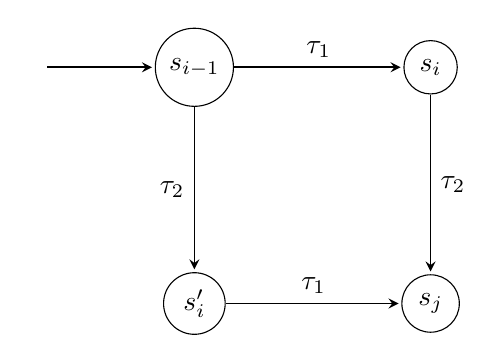
\begin{tikzpicture}
    [pre/.style={<-,shorten <=1pt,>=stealth,semithick}]
    \node (A) at (0,0) {};
    \node [shape=circle,draw=black] (B) at (2, 0) {\(s_{i-1}\)}
      edge [pre] node[above] {} (A);
    \node [shape=circle,draw=black] (C) at (2, -3) {\(s_i'\)}
      edge [pre] node[left] {\(\tau_2\)} (B);
    \node [shape=circle,draw=black] (D) at (5, 0) {\(s_i\)}
      edge [pre] node[above] {\(\tau_1\)} (B);
    \node [shape=circle,draw=black] (E) at (5, -3) {\(s_j\)}
      edge [pre] node[right] {\(\tau_2\)} (D)
      edge [pre] node[above] {\(\tau_1\)} (C);
  \end{tikzpicture}
  \caption{Influence of the order of independent transitions on the global state of an evaluation engine}
\label{fig:chap4:sec_run:exchange_transitions}
\end{figure}

\begin{lemma}[name = Duration of Enabledness]\label{lemma:enabled_till_scheduled}
  A node which is enabled stays enabled at least until it is scheduled.
  Formally: If a node \(n\) is enabled at step \(i\) in a run \(r\) it will stay enabled at least until the first step \(j > i\) with \(r(j) = (\tau,s), \mathit{node}(\tau) = n\).
  Note that it doesn't have to be disabled after step \(j\), because there could have been multiple events buffered on it's inputs.
\end{lemma}

\begin{proof}
  Let \(n\) be a node enabled at step \(i\) in a run \(r\).
  Let \((\tau_x,s_x) = r(x), x = i + 1\).
  If \(\mathit{node}(\tau_x) \neq n\), then the only influence that \(\tau_x\) can have on the node state \(\widetilde{n}\) of \(n\) is by appending produced events to one of the input queues, as per the definition of application of a transition.
  Since \(\tau_x\) can't remove events from the input queues in \(\widetilde{n}\) and on all input queues was at least one event buffered before the transition was applied, else \(n\) wouldn't have been enabled at step \(i\), \(\widetilde{n}\) will have at least as many input events buffered on every input as in the step before.
  This means that \(n\) is still enabled at step \(x\), and by induction at every later step until a transition with \(n\) as its node is taken.
\end{proof}

\begin{lemma}[name = Finiteness of Enabledness]\label{lemma:finiteness_enabledness}
  Whenever a node is enabled in a run, it can only be scheduled continously a limited number of times until becoming disabled.
\end{lemma}

\begin{proof}
  Let \(n\) be an enabled node at step \(i\) with the node state \(\widetilde{n}\).
  First let's assume that no parent of \(n\) are scheduled after step \(i\) and before \(n\) becomes disabled.
  Since the input queues of \(n\) are filled by previous transitions and only finite number of events are produced at every step, all of the queues can only have a finite number of events buffered at step \(i\).
  Since no parents of \(n\) are scheduled, the queues can't get fuller.
  Because all nodes represent functions, and all functions have to consume at least one input event (compare \Cref{sec:definitions:tessla_functions}), everytime \(n\) is scheduled at least one input queue of \(n\) will have one event less buffered after it performed its computation.
  Therefore the worst case is when \(n\) only consumes one event per computation.
  The maximum number of time \(n\) can be scheduled is therefore bounded by the sum of the number of events on all input queues at step \(i\).

  Now let's assume that also input nodes of \(n\) can be scheduled after step \(i\).
  Everytime an input node is scheduled it will add a finite amount of events to one input queue of \(n\).
  This leads to a cyclic behaviour: If an input queue can be scheduled infinitely often, infinite many events will be added to the input queue and \(n\) can possibly be scheduled infinitely often.
  If input queues can not compute infinitely often, only a finite amount of events are added to the inputs of \(n\) and therefore \(n\) can only be scheduled a limited number of times.
  Closer inspection of the nature of evaluation engines show why this is no problem: Only if the external trace fed to an evaluation engine is infinte the source nodes can compute infintely often.
  Hence for finite traces no node can compute infinitely often.
  Again the worst case is when \(n\) only consumes one event per computation.
  The number of times it can be scheduled is limited by the sum of the number of events buffered on the inputs at step \(i\) and the number of events that are produced by inputs of \(n\) after step \(i\).
\end{proof}

With the notion of runs and especially enabledness we can now define which schedules are seen as fair.

\begin{definition}[name = Fair Schedules]\label{def:fair_schedule}
  A schedule of an evaluation engine is called fair, if for all runs \(r\)  it produces the following holds:
  \begin{align*}
    &\forall i < \mathit{length}(r):\ &&\text{if }n\ \text{is enabled at step } i\\
    &                                 &&\text{then } \exists\, j \geq i\ \text{such that n is scheduled at step } j
\end{align*}
In other words, every enabled node is scheduled after a finite number of steps.
\end{definition}

Building on this we will investigate different fair schedules in the next chapter.
